\chapter{网络编程}

\section{计算机网络}

\subsection{网络}

对于现代的程序开发来讲,几乎都是面向于网络的应用环境,包括程序项目开发也完全离不开网络。例如使用Python开发就一定会需要通过pip下载相应的模块组件。\\

世界上最早出现的计算机是为了解决数据的计算以及密码的破译,如果继续延伸也都是军方进行数据存储的重要的技术研究。而后计算机开始进入到普通平民的生活,当有了多台电脑之后肯定需要想办法把这多台电脑进行连接,于是就有了局域网。世界上的人们都想要进行连接,那么就需要创建互联网。\\

两台主机通讯一定要保证所有的网络线路是通畅的,协议指的是双方必须遵守的共同约定,在进行网络通讯的时候实际上核心的功能就是I/O操作。\\

\subsection{网络程序开发模式}

在进行网络程序开发的过程之中一般都会考虑两种不同的开发模式:

\begin{itemize}
	\item C/S模式(Client / Server,客户端与服务端架构):该设计架构一般需要编写两套不同的程序,一套是服务端程序,另一套是客户端程序。在进行项目维护的时候需要进行两套项目的维护,所以维护成本很高。但是这种程序一般使用特定的协议、特定的数据结构、影藏的端口等,所以安全性是比较高的。

	\item B/S模式(Browser / Server,浏览器与服务端架构):主要是基于WEB设计的一种架构,基于浏览器的形式作为客户端进行访问。在程序开发的时候只开发一套服务端即可,所以开发的成本比较低,而且用户使用门槛页比较低。但是这种开发一般都是基于HTTP协议完成的,所以其安全性不高,因为使用的是公共的80端口,极易遭到攻击。
\end{itemize}

\vspace{0.5cm}

\subsection{OSI七层模型}

对于网络程序的开发不仅仅是一个简单的数据交换的过程,还包含一些数据的处理逻辑,同时所有的网络设备也一定会由不同的硬件产商生产。所以为了可以保证数据传输的可靠性以及标准型,就定义了OSI(Open System Interconnection)七层模型。

\begin{table}[H]
	\centering
	\setlength{\tabcolsep}{5mm}{
		\begin{tabular}{|c|l|}
			\hline
			\textbf{协议层} & \textbf{功能}                         \\
			\hline
			应用层          & 提供网络服务操作接口                  \\
			\hline
			表示层          & 对要传输的数据进行处理                \\
			\hline
			会话层          & 管理不同通讯节点之间的连接信息        \\
			\hline
			传输层          & 建立不同结点之间的网络连接            \\
			\hline
			网络层          & 将网络地址映射为MAC地址实现数据包转发 \\
			\hline
			数据链路层      & 将要发送的数据包转为数据帧            \\
			\hline
			物理层          & 利用物理设备实现数据的传输            \\
			\hline
		\end{tabular}
	}
	\caption{OSI七层模型}
\end{table}

由于有了这七层不同的网络数据的处理分类,所以任何的硬件产商生产的设备,其核心的处理本质都不会发生改变。\\

Python属于高级语言,所以对于所有的网络程序开发不可能让开发者自行处理具体的OSI模型,应该采用统一的模式进行定义,这样就有了Socket编程。

\begin{figure}[H]
	\centering
	\begin{tikzpicture}
		\draw (0,0) rectangle (3,7);
		\draw (8,0) rectangle (11,7);
		\draw (0,1) -- (3,1);
		\draw (0,2) -- (3,2);
		\draw (0,3) -- (3,3);
		\draw (0,4) -- (3,4);
		\draw (0,5) -- (3,5);
		\draw (0,6) -- (3,6);
		\draw (8,1) -- (11,1);
		\draw (8,2) -- (11,2);
		\draw (8,3) -- (11,3);
		\draw (8,4) -- (11,4);
		\draw (8,5) -- (11,5);
		\draw (8,6) -- (11,6);

		\draw (1.5,6.5) node{应用层};
		\draw (1.5,5.5) node{表示层};
		\draw (1.5,4.5) node{会话层};
		\draw (1.5,3.5) node{传输层};
		\draw (1.5,2.5) node{网络层};
		\draw (1.5,1.5) node{数据链路层};
		\draw (1.5,0.5) node{物理层};
		\draw (9.5,6.5) node{应用层};
		\draw (9.5,5.5) node{表示层};
		\draw (9.5,4.5) node{会话层};
		\draw (9.5,3.5) node{传输层};
		\draw (9.5,2.5) node{网络层};
		\draw (9.5,1.5) node{数据链路层};
		\draw (9.5,0.5) node{物理层};

		\draw[->, very thick] (-1,7) -- (-1,0);
		\draw[->, very thick] (12,0) -- (12,7);
		\draw[->] (1.5,0) -- (1.5,-1) -- (9.5,-1) -- (9.5,0);
	\end{tikzpicture}
	\caption{数据传输}
\end{figure}

\subsection{Socket}

Socket(套接字)是一种对TCP网络协议进行的一种包装(协议的抽闲应用),它本身最大的特点是提供了不同进行之间的数据通讯操作。所有的网络协议的组成是非常繁琐的,如果所有的开发者去研究具体的通讯协议会对开发带来很大的难度,所以在不同的编程语言内部就会考虑对一些网络的协议进行包装。\\

Socket主要是真对两种协议的包装:

\begin{itemize}
	\item TCP(Transmission Control Protocol传输控制协议):采用有状态的通讯机制进行传输,在通讯时会通过三次握手机制保证与一个指定节点的数据传输的可靠性,在通讯完毕后会通过四次挥手的机制关闭连接。由于在每次数据通讯前都需要消耗大量的时间进行连接控制,所以执行性能较低,且系统资源占用较大。

	\item UDP(User Datagram Protocol用户数据报协议):采用无状态的通讯机制进行传输,没有了TCP中复杂的握手与挥手处理机制,这样就节约了大量的系统资源,同时数据传输性能较高。但是由于不保存单个节点的连接状态,所以发送的数据不一定可以被全部接收。UDP不需要连接就可以直接发送数据,并且多个接收端都可以接收同样的消息,所以使用UDP适合于广播操作。
\end{itemize}

\newpage

\section{TCP / UDP}

\subsection{TCP}

在网络编程之中,TCP属于面向连接的通讯协议,所以在进行TCP通讯的过程之中其安全性以及稳定性都是最高的,虽然性能会差一些,但是对于当前网络环境来讲主要使用的还是TCP协议居多。\\

在Python里面提供有一个socket.socket类可以实现TCP的程序编写。

\begin{table}[H]
	\centering
	\setlength{\tabcolsep}{5mm}{
		\begin{tabular}{|l|l|}
			\hline
			\textbf{方法}             & \textbf{功能}                        \\
			\hline
			socket()                  & 获取socket类对象                     \\
			\hline
			bind((hostname, port))    & 在指定主机的端口绑定监听             \\
			\hline
			listen()                  & 在绑定端口上开启监听                 \\
			\hline
			accpet()                  & 等待客户端连接,连接后返回客户端地址 \\
			\hline
			send(data)                & 发送数据                             \\
			\hline
			recv(buffer)              & 接收数据                             \\
			\hline
			close()                   & 关闭套接字连接                       \\
			\hline
			connect((hostname, port)) & 设置要连接的主机名称和端口号         \\
			\hline
		\end{tabular}
	}
	\caption{socket.socket类}
\end{table}

在整个Socket通讯过程之中,由于其属于C/S程序结构,所以一定要开发两套程序。对于服务器端程序来讲一定要在特定的主机端口上开启监听机制,这样客户端就可以依据服务器的地址和端口进行服务的访问。

\begin{figure}[H]
	\centering
	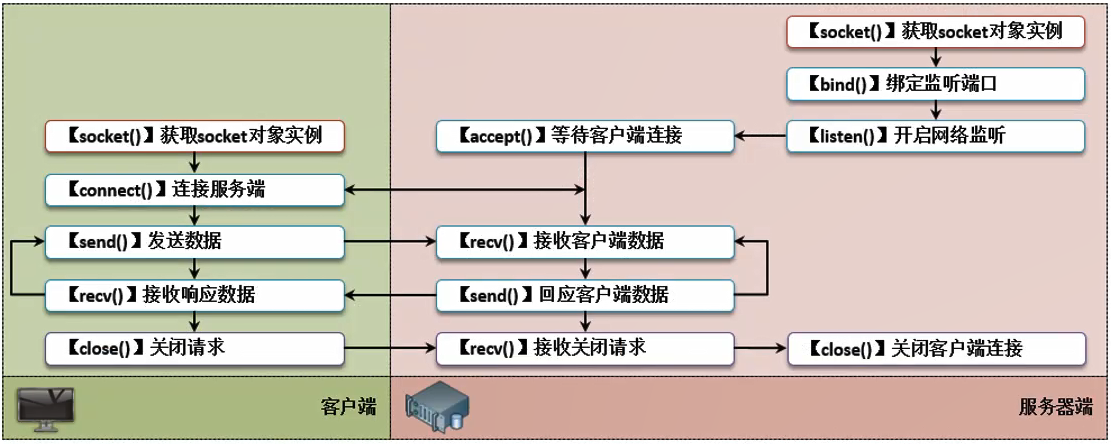
\includegraphics[scale=0.6]{img/C12/12-2/1.png}
	\caption{TCP}
\end{figure}

\vspace{0.5cm}

\mybox{TCP}

\begin{lstlisting}[language=Python, title=tcp\_server.py]
import socket

SERVER_HOST = "localhost"   # 127.0.0.1(本机IP)
SERVER_PORT = 8080

def main():
    # 获取socket对象
    with socket.socket() as sock:
        # 绑定本机的8080端口
        sock.bind((SERVER_HOST, SERVER_PORT))
        sock.listen()   # 开启监听
        print("【服务端】服务器启动完毕。")
        print("【服务端】等待客户端连接...")

        # 当有客户端连接后,获取客户端的socket和地址
        client, client_addr = sock.accept()
        with client:
            print("【服务端】客户端%s (port: %s)连接到服务器"
                    % client_addr)
            while True:     # 持续接收和响应信息
                # 接收客户端发送的数据
                data = client.recv(100).decode("UTF8")
                print("【服务端】接收数据:%s" % data)
                if data == "exit":      # 客户端发送退出指令
                    # 向客户端发送响应
                    client.send("exit".encode("UTF8"))
                    break
                else:
                    client.send(
                        ("【服务端】%s" % data).encode("UTF8")
                    )

if __name__ == "__main__":
    main()
\end{lstlisting}

所有的网络程序一定要有一个绑定的端口,所以一个端口只允许绑定一套服务,如果出现了端口被占用的情况,那么程序将无法正常启动。如果出现重复绑定的问题会出现Exception has occurred: OSError错误提示。\\

由于该程序是由标准的TCP协议实现,所以可以直接使用telnet命令连接服务器:

\vspace{-0.5cm}

\begin{lstlisting}
telnet localhost 8080
\end{lstlisting}

如果没有安装telnet,需要进入【Windows功能】进行手动安装。但telnet属于操作系统提供的一个测试命令,并不能作为实际的程序客户端使用,那么就需要开发自己的Socket客户端。

\begin{figure}[H]
	\centering
	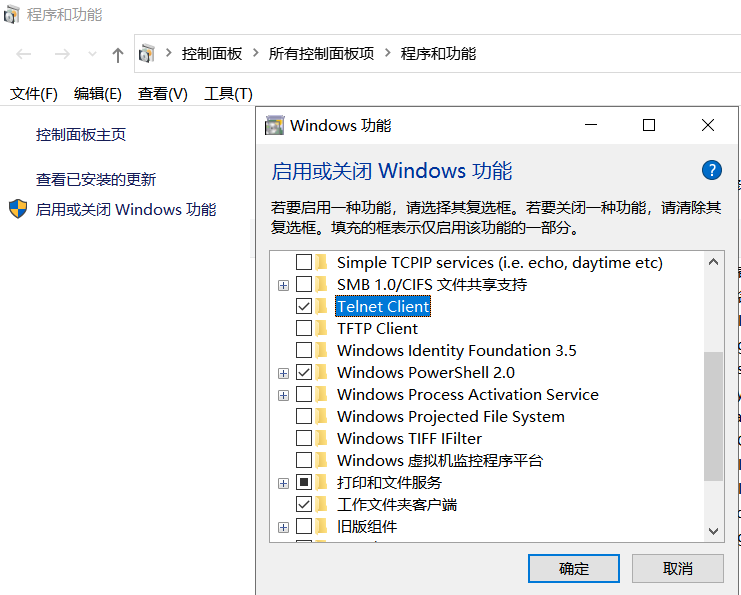
\includegraphics[scale=0.7]{img/C12/12-2/2.png}
\end{figure}

\begin{lstlisting}[language=Python, title=tcp\_client.py]
import socket

SERVER_HOST = "localhost"   # 服务器端IP地址
SERVER_PORT = 8080          # 服务器连接端口

def main():
    # 获取socket对象
    with socket.socket() as sock:
        # 连接服务器
        sock.connect((SERVER_HOST, SERVER_PORT))
        
        while True:     # 客服端持续与服务端交互
            msg = input("【客户端】输入数据:")
            sock.send(msg.encode("UTF8"))
            reply = sock.recv(100).decode("UTF8")
            if reply == "exit":
                break
            else:
                print(reply)

if __name__ == "__main__":
    main()
\end{lstlisting}

\vspace{0.5cm}

\subsection{UDP}

UDP也是工作在传输层上的协议,但是与TCP相比,UDP本身采用的是不安全的连接,所以每次通过UDP发送的数据不一定可以接收到,但是其性能比较好。\\

Python中对于TCP和UDP本身的实现结构差别不大,都是通过socket.socket类完成的,只需要设置一些参数即可。\\

UDP服务端与TCP最大的区别在于不再需要过多的考虑到数据稳定性的连接问题,所以也不再设置具体的监听操作。在每次接收到请求之后只需要获取客户端的原始地址,直接原路返回即可。

\newpage